Polar Orbits are probably the simplest way to configure an evenly spaced constellation. As we will see in the section \textbf{Orbit Perturbations} when the inclination is the same for all the planes, the deviations tend to be the same for all the satellites. An example of near polar orbits is the constellation Iridium \cite{Iridium}. You can find the example in detail in [{REF TO ANNEX I. Section 3.2}]

\subsubsubsection*{General Configuration}
\begin{minipage}{0.45\textwidth}
The Polar Orbits configuration consists in the distribution of plains with inclination equal to 90 degrees. Note that the satellites will be travelling parallel to the satellites of the next plain except for the communications between the first and the last plane, hence the separation between this two is smaller. The plains are splitted in the pattern of figure \cite{fig:polardist}:
\end{minipage}
\vline
\begin{minipage}{0.45\textwidth}
\begin{figure}[H]\label{fig:polardist}
\begin{center}
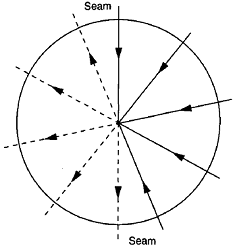
\includegraphics[scale=0.40]{PolarOrbits/planeconfig.png}
\caption{Distribution of the planes for Polar Orbits design.}
\end{center}
\end{figure}

\end{minipage}

\subsubsubsection*{The Streets of Coverage Method}
The Street of Coverage Method is a way to compute the necessary plains and satellites to construct a Polar Orbit Constellation that provides global coverage. It is obtained from 
\cite{Chobotov2002} and described in 
[{REF TO ANNEX I. Section 3.3}]

\textbf{Results of the Streets of Coverage Method\\}
A MATLAB routine detailed in [{REF TO ANNEX VII. Satellite Number Computation for Polar Orbits}] has been designed to compute the  algorithm. The program is runned in a broad range of parameters to see the evolution of the number of satellites. As it can be predicted, as the height increases the number of satellites is reduced. The reason is that the footprint of the satellites increases with the height. In addition, as the minimum elevation over the horizon to contact the satellites is reduced, the number of satellites is also reduced for the same reason. 

\begin{figure}[H]
\begin{center}
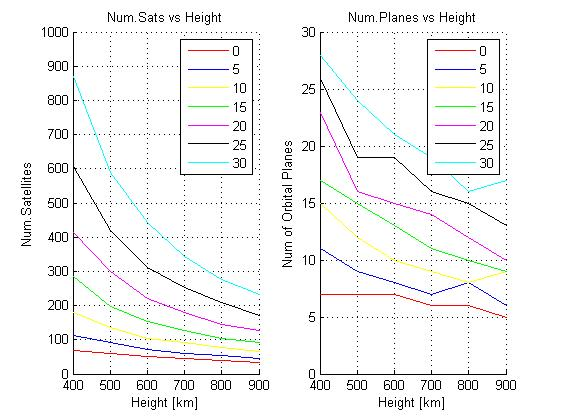
\includegraphics[scale=0.6]{PolarOrbits/GeneralResults.jpg}
\caption{Variation of number of satellites for different heights and elevation angles}
\end{center}
\end{figure}

%\textbf{Detailed Solution}\\
%Given the previously justified assumptions, the same simulation is computed for a more reasonable range of results. In this case, the elevation is set as: $$\varepsilon = 20º$$.
%
%\begin{figure}[H]
%\begin{center}
%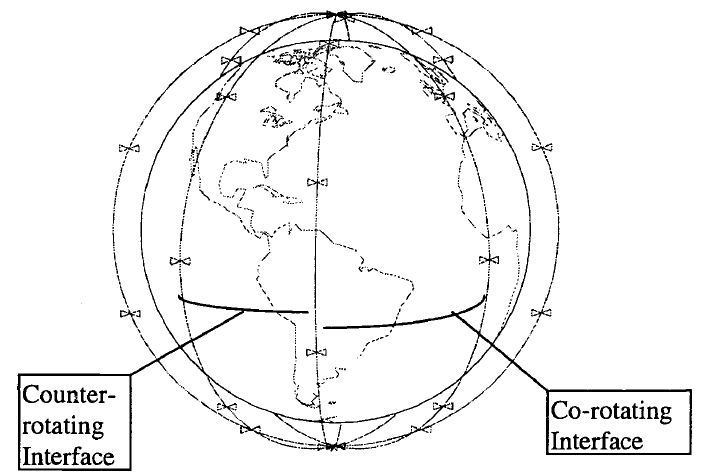
\includegraphics[scale=0.7]{PolarOrbits/Polar.jpg}
%\caption{Variation of number of satellites for different heights between 500 and 600km.}
%\end{center}
%\end{figure}

\textbf{Conclusion}\\
The computation and the design of this constellation requires small computational and conceptual effort. However, the number of satellites and planes is greater than expected. Even though the technical complexity can be reduced, the availability of small launchers to reach this particularly inclined orbit is also small. In conclusion, more constellation configurations need to be assessed to compare and select the most feasible one.

%\bibliographystyle{unsrt}
%\bibliography{forouzan,Secretariat2014,TC,tmsynch,OrbitalMechanics
%\end{document}